\chapter{ Classification par réseau convolutif (CNN)}



\section{Architecture du Modèle CNN}

Le réseau est structuré en quatre blocs convolutifs dont le nombre de filtres double
à chaque niveau, permettant une extraction hiérarchique de caractéristiques de plus en
plus abstraites :
\begin{figure}[H]
\centering
    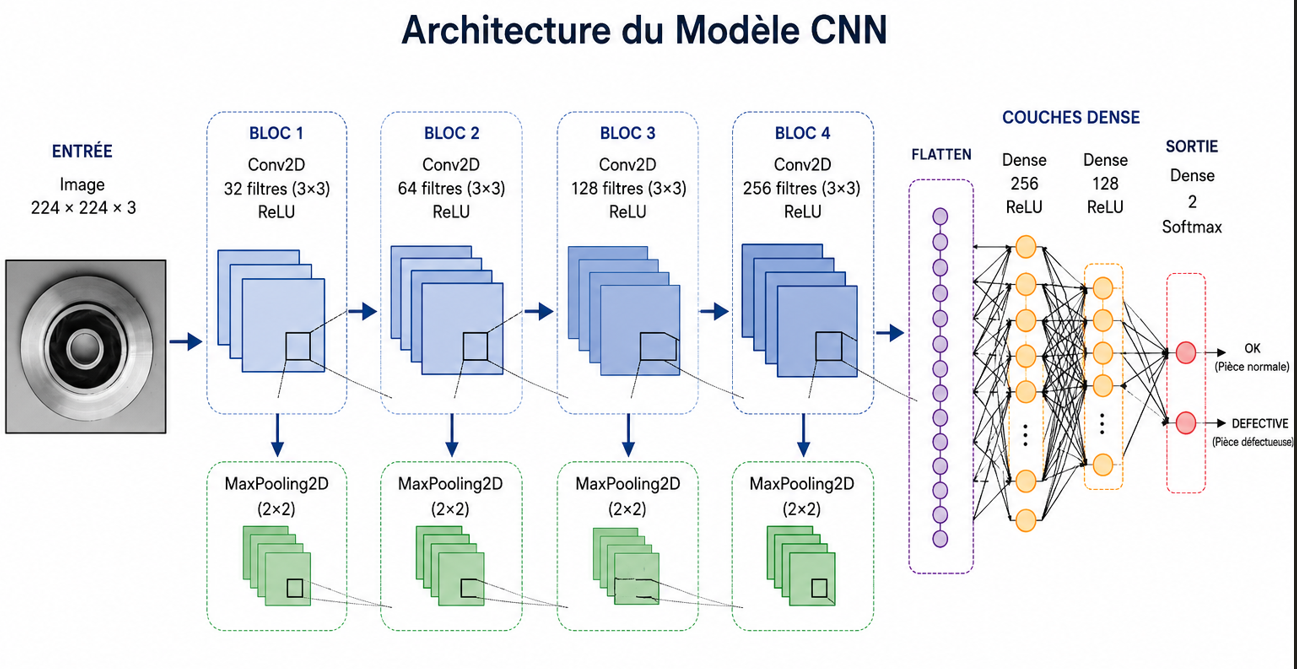
\includegraphics[width=0.8\linewidth]{archi.png}
    \caption{Architecture du CNN}
\end{figure}

\subsection{Convolution 2D}

L'opération de convolution est définie par :

\begin{equation}
(I * K)[i,j] = \sum_{m}\sum_{n} I[i+m,\, j+n] \cdot K[m,n]
\end{equation}

Tous les filtres utilisent un \textit{padding} de type \texttt{same},
préservant les dimensions spatiales à travers chaque couche convolutive
avant le sous-échantillonnage.

\subsubsection{Activation ReLU}

La fonction d'activation \term{ReLU} (\textit{Rectified Linear Unit}) est
utilisée pour introduire la non-linéarité :

\begin{equation}
\text{ReLU}(x) = \max(0, x)
\end{equation}

Son avantage principal est de ne pas saturer pour les grandes valeurs positives,
limitant le problème du gradient qui s'éteint (\textit{vanishing gradient}).

\subsubsection{MaxPooling}

Chaque bloc se termine par un sous-échantillonnage spatial $2 \times 2$ par
maximum local, réduisant de moitié les dimensions spatiales tout en conservant
les caractéristiques les plus saillantes :

\begin{equation}
\text{Sortie}_{i,j} = \max_{(p,q) \in \mathcal{P}_{i,j}} x_{p,q}
\end{equation}

Après les quatre blocs, les cartes de caractéristiques ont des dimensions
$14 \times 14 \times 256$.

\section{Classifieur dense}

La tête de classification comprend deux couches denses avec régularisation,
suivies d'une sortie \term{softmax} :

\begin{align}
h_1 &= \text{ReLU}(\text{}(W_1 \cdot \text{Flatten}(x) + b_1)) \\
h_2 &= \text{ReLU}(\text{}(W_2 \cdot h_1 + b_2)) \\
\hat{y} &= \text{softmax}(W_3 \cdot h_2 + b_3)
\end{align}

La sortie \texttt{softmax} fournit une distribution de probabilité sur les
deux classes :

\begin{equation}
\text{softmax}(z_i) = \frac{e^{z_i}}{\sum_{j} e^{z_j}}
\end{equation}


\section{Régularisation du Modèle}
% =============================================================

\subsection{Stratégies de régularisation employées}

Le premier modèle (\model{CNN\_REG}) intègre deux techniques de régularisation
complémentaires : la \term{Batch Normalization} et le \term{Dropout}.

\subsection{Batch Normalization}

la Batch Normalization
normalise les activations de chaque couche par lot pendant l'entraînement :

\begin{equation}
\hat{x}^{(k)} = \frac{x^{(k)} - \mu_{\mathcal{B}}^{(k)}}{\sqrt{\sigma_{\mathcal{B}}^{(k)2} + \epsilon}}
\end{equation}

puis applique une transformation affine apprise :

\begin{equation}
y^{(k)} = \gamma^{(k)} \hat{x}^{(k)} + \beta^{(k)}
\end{equation}

\textbf{Avantages dans ce contexte :}
\begin{itemize}
  \item Accélère la convergence en réduisant le \term{covariate shift} interne ;
  \item Agit comme régularisateur implicite, réduisant le besoin de Dropout
        dans les couches convolutives ;
  \item Permet l'utilisation de taux d'apprentissage plus élevés.
\end{itemize}

La Batch Normalization est appliquée \textbf{après} chaque couche convolutive et \textbf{après}
les couches denses, avant l'activation (pattern BN-avant-activation).

\subsection{Dropout}

Le Dropout désactive aléatoirement des neurones pendant
l'entraînement avec une probabilité $p$, forçant le réseau à apprendre des
représentations redondantes et robustes 
\begin{table}[H]
\centering
\caption{Paramètres de Dropout dans le classifieur}
\label{tab:dropout}
\begin{tabular}{|l|c|p{8cm}|}
\toprule
\textbf{Couche} & \textbf{Taux de Dropout} & \textbf{Justification} \\
\midrule
Dense(256) & $p = 0{,}5$ & Fort : couche la plus dense, risque élevé de sur-apprentissage \\
\hline
Dense(128) & $p = 0{,}3$ & Modéré : couche intermédiaire \\
\bottomrule
\end{tabular}
\end{table}


\subsection{Code complet (Modèle CNN régularisé)}

\begin{figure}[H]
\centering
    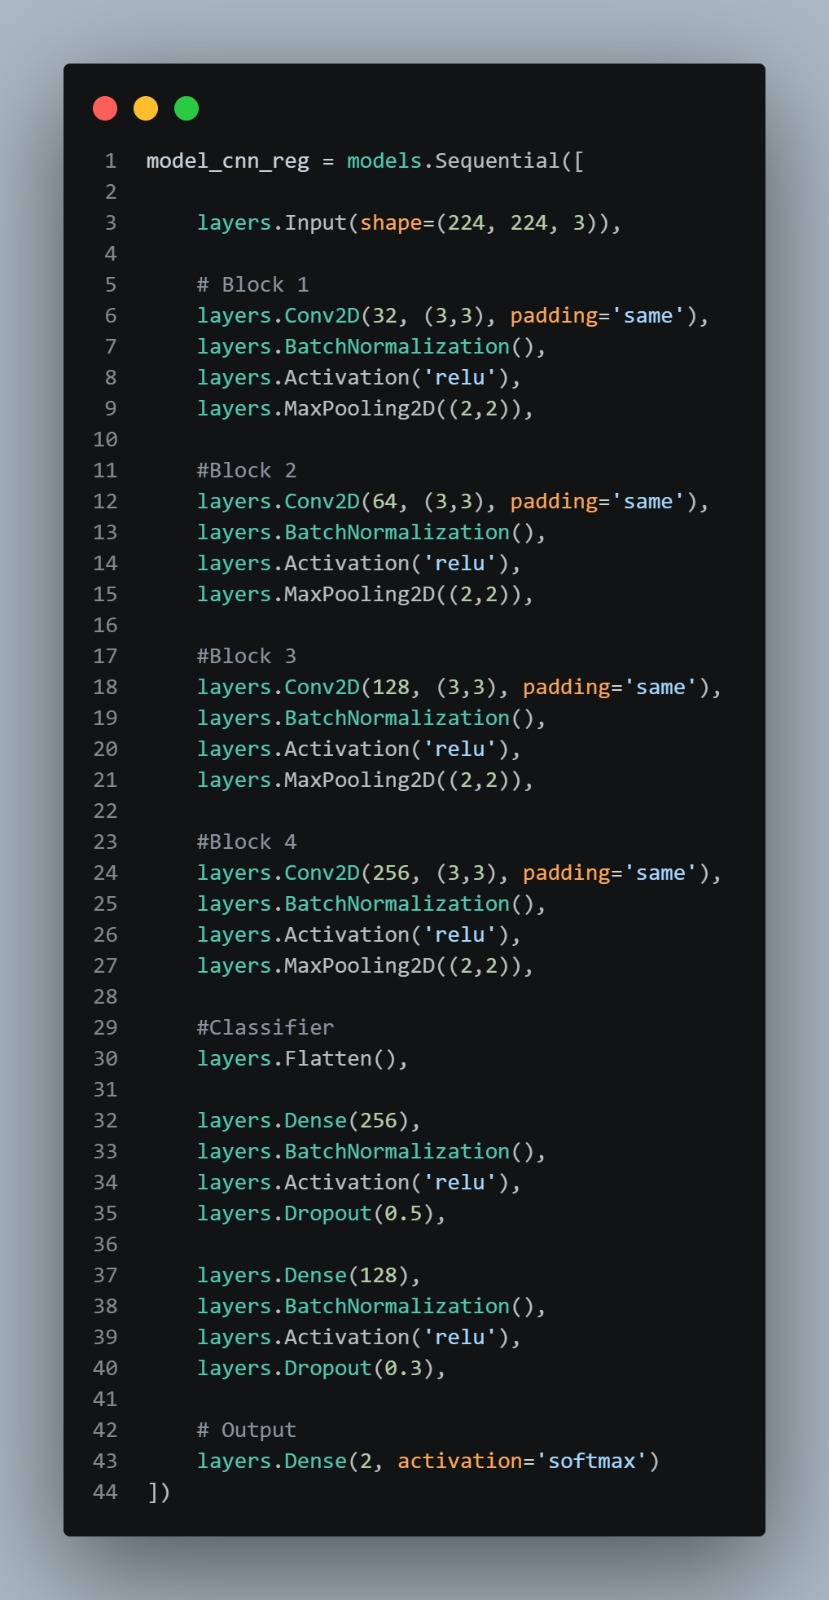
\includegraphics[width=0.8\linewidth]{code1.jpeg}
    \caption{}
\end{figure}


\newpage

\section{Récapitulatif de l'architecture}






\begin{table}[H]
\centering
\caption{Récapitulatif complet de l'architecture CNN régularisé}
\label{tab:archi}
\renewcommand{\arraystretch}{1.3}
\begin{tabular}{|c|l|c|c|}
\hline
\textbf{Bloc} & \textbf{Couche} & \textbf{Filtres / Unités} & \textbf{Sortie} \\
\hline
Input & Input & --- & $224 \times 224 \times 3$ \\
\hline
\multirow{1}
    & Conv2D    & $32,\ 3\times3$ & $224\times224\times32$ \\
    & BatchNorm & ---             & $224\times224\times32$ \\
    & ReLU      & ---             & $224\times224\times32$ \\
    & MaxPool2D & $2\times2$      & $112\times112\times32$ \\
\hline
\multirow{2}
    & Conv2D    & $64,\ 3\times3$ & $112\times112\times64$ \\
    & BatchNorm & ---             & $112\times112\times64$ \\
    & ReLU      & ---             & $112\times112\times64$ \\
    & MaxPool2D & $2\times2$      & $56\times56\times64$   \\
\hline
\multirow{3}
    & Conv2D    & $128,\ 3\times3$ & $56\times56\times128$ \\
    & BatchNorm & ---              & $56\times56\times128$ \\
    & ReLU      & ---              & $56\times56\times128$ \\
    & MaxPool2D & $2\times2$       & $28\times28\times128$ \\
\hline
\multirow{4}
    & Conv2D    & $256,\ 3\times3$ & $28\times28\times256$ \\
    & BatchNorm & ---              & $28\times28\times256$ \\
    & ReLU      & ---              & $28\times28\times256$ \\
    & MaxPool2D & $2\times2$       & $14\times14\times256$ \\
\hline
--- & Flatten   & ---    & $50\,176$ \\
\hline
\multirow{FC}
    & Dense          & 256       & 256 \\
    & BatchNorm+ReLU & ---       & 256 \\
    & Dropout        & $p=0{,}5$ & 256 \\
    & Dense          & 128       & 128 \\
    & BatchNorm+ReLU & ---       & 128 \\
    & Dropout        & $p=0{,}3$ & 128 \\
\hline
Output & Dense (softmax) & 2 & 2 \\
\hline
\end{tabular}
\end{table}






\newpage

\section{Méthodologie d'Entraînement}

\subsection{Fonction de perte}

La fonction de perte utilisée est la \term{Cross-Entropie Catégorielle
Parcimonieuse} (\textit{Sparse Categorical Cross-Entropy}), adaptée aux
labels entiers :

\begin{equation}
\mathcal{L}(\theta) = -\frac{1}{N}\sum_{i=1}^{N} \log \hat{y}_{i, y_i}
\end{equation}

où $\hat{y}_{i, y_i}$ est la probabilité prédite pour la vraie classe $y_i$
de l'exemple $i$.

\subsection{Optimiseur}

L'algorithme \textbf{Adam} est choisi pour ses propriétés
de convergence adaptative. Il combine les avantages de RMSProp (adaptation
du taux d'apprentissage par paramètre) et Momentum 



\subsection{Stratégie d'arrêt précoce}

L'\term{Early Stopping} est mis en place pour interrompre l'entraînement
dès que la performance sur le jeu de validation stagne, prévenant le
sur-apprentissage

\begin{figure}[H]
\centering
    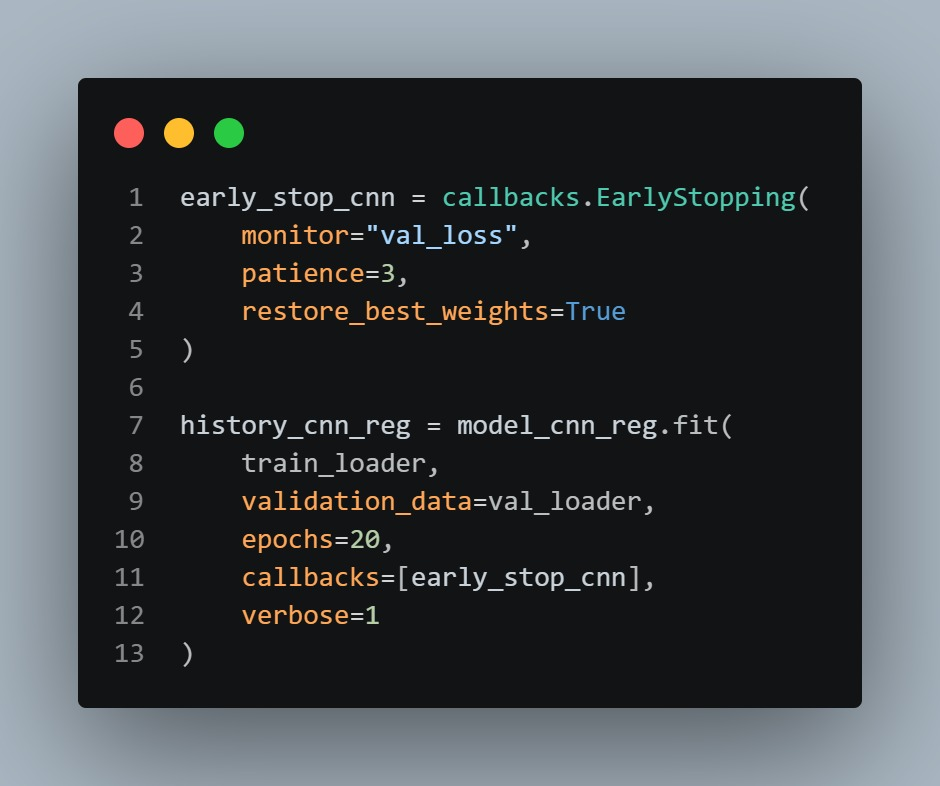
\includegraphics[width=0.8\linewidth]{code2.jpeg}
    \caption{Architecture du CNN}
\end{figure}


\subsection{Paramètres d’entraînement récapitulatifs}

\begin{table}[H]
\centering
\caption{Hyperparamètres d'entraînement communs aux deux modèles}
\label{tab:hyperparam}
\begin{tabular}{|l|l|}
\hline
\textbf{Hyperparamètre} & \textbf{Valeur} \\
\hline
Optimiseur        & Adam  \\
\hline
Fonction de perte & Sparse Categorical Cross-Entropy \\
\hline
Métrique          & Accuracy \\
\hline
Batch size        & 32 \\
\hline
Époques max       & 20 \\
\hline
Résolution        & $224 \times 224 \times 3$ \\
\hline


\end{tabular}
\end{table}


\section{Modèle CNN sans Augmentation — Résultats}

\subsection{Courbes d'apprentissage}

Les courbes d'apprentissage illustrent
l'évolution de la précision et de la perte sur les ensembles
d'entraînement et de validation au fil des époques.

\begin{figure}[H]
\centering
    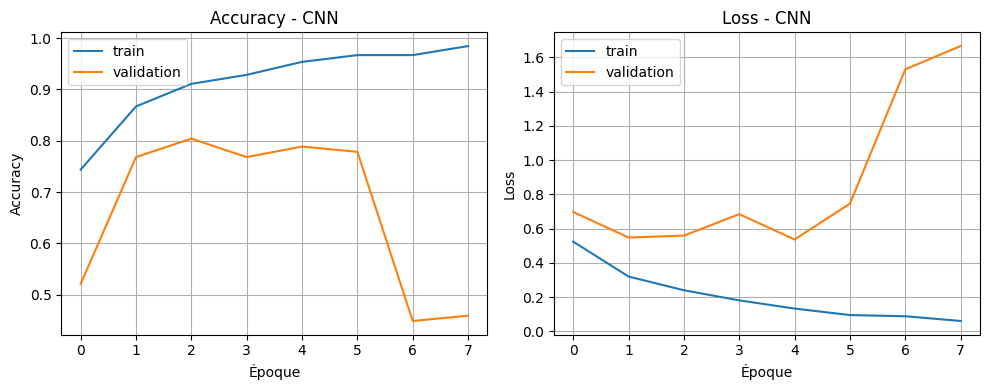
\includegraphics[width=0.8\linewidth]{code3.png}
    \caption{Courbes d'apprentissage}
\end{figure}

\subsection{Lecture des courbes}
- La courbe train (bleue) progresse de manière régulière et quasi-monotone, partant de ~0,74 à l'époque 0 pour atteindre ~0,97 à l'époque 7.

- La courbe validation (orange) démarre à ~0,52, monte rapidement jusqu'à ~0,80 aux époques 2–3, se stabilise autour de 0,78–0,80 jusqu'à l'époque 5, puis s'effondre brutalement à ~0,45 aux époques 6–7.

- La loss d'entraînement (bleue) décroît de façon continue et régulière, de ~0,55 à quasi 0,05 à l'époque 7, une descente quasi-parfaite.

- La loss de validation (orange) oscille entre 0,55 et 0,65 jusqu'à l'époque 4, puis diverge fortement pour atteindre ~1,65 à l'époque 7.

\subsection{Interprétation :}

- Le creusement progressif entre les deux courbes à partir de l'époque 3 est un signal clair de sur-apprentissage (overfitting) : le modèle mémorise les données d'entraînement sans généraliser.

- L'effondrement brutal de la validation aux époques 6–7 confirme que le modèle a dépassé son optimum de généralisation bien avant la fin de l'entraînement.

- La divergence entre la loss train et la loss validation à partir de l'époque 5 est le symptôme classique du sur-apprentissage : la perte d'entraînement continue de baisser alors que la perte de validation explose.

- Le minimum de la loss de validation se situe vers l'époque 4 (~0,57), confirmant que c'est le point optimal d'arrêt.

- La forte amplitude des oscillations sur la courbe de validation (notamment la chute aux époques 6–7 sur l'accuracy) suggère une instabilité du modèle face aux données non vues, probablement amplifiée par l'absence d'augmentation de données.

\subsection{ Conclusion générale :}

Malgré la présence de Batch Normalization et de Dropout, le modèle CNN régularisé entre en sur-apprentissage dès l'époque 5, atteignant une précision de validation maximale d'environ 80\%. Ce comportement motive directement l'introduction de l'augmentation de données dans le second modèle, afin d'enrichir artificiellement la diversité des exemples d'entraînement et de retarder — voire d'éliminer — ce phénomène de sur-apprentissage.

\subsection{Résultats sur l’ensemble de test}

\begin{table}[H]
\centering
\caption{Résultats d'évaluation du modèle CNN régularisé sur l'ensemble de test}
\label{tab:test_results_reg}
\begin{tabular}{|l|c|}
\hline
\textbf{Métrique} & \textbf{Valeur} \\
\hline
Test Loss     & $62{,}29\%\\
\hline
Test Accuracy & $80{,}20\%$ \\
\hline
\end{tabular}
\end{table}

\subsection{Matrice de confusion}

\begin{figure}[H]
\centering
    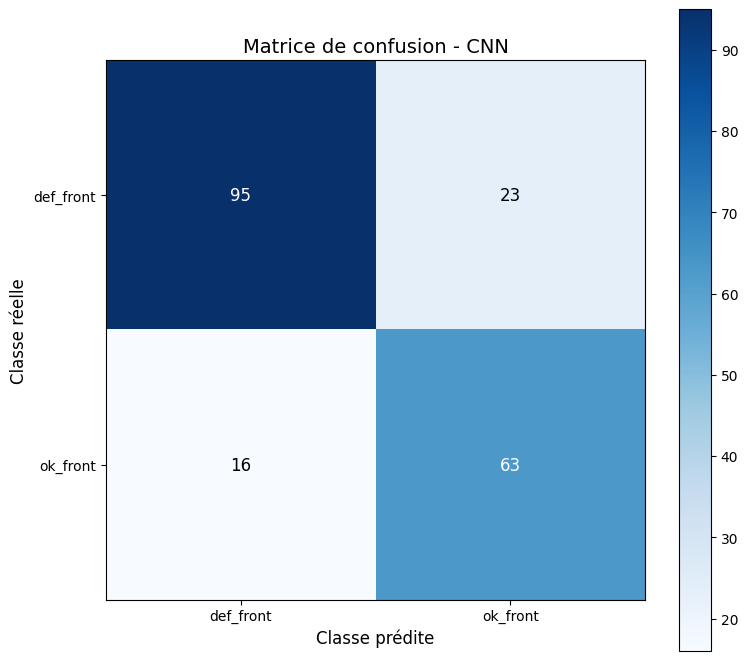
\includegraphics[width=0.8\linewidth]{code4.png}
    \caption{Matrice de confusion}
\end{figure}


La matrice de confusion permet d'analyser la
nature des erreurs du modèle. On distingue :
\begin{itemize}
  \item \textbf{Vrais Positifs (TP)} : 95 pièces défectueuses correctement identifiées.
  \item \textbf{Vrais Négatifs (TN)} : 63 pièces saines correctement identifiées.
  \item \textbf{Faux Positifs (FP)} : 16 pièces saines classées comme défectueuses.
  \item \textbf{Faux Négatifs (FN)} : 23 pièces défectueuses classées comme saines (\textit{défaut non détecté}).
\end{itemize}


\subsection{Rapport de classification}

\begin{table}[H]
\centering
\caption{Rapport de classification — CNN régularisé (sans augmentation)}
\label{tab:report_reg}
\renewcommand{\arraystretch}{1.3}
\begin{tabular}{|l|c|c|c|c|}
\hline
\textbf{Classe} & \textbf{Précision} & \textbf{Rappel} & \textbf{F1-Score} & \textbf{Support} \\
\hline
\texttt{def\_front}      & $0{,}86$ & $0{,}81$ & $0{,}83$ & 118 \\
\hline
\texttt{ok\_front}       & $0{,}73$ & $0{,}80$ & $0{,}76$ & 79  \\
\hline\hline
\textbf{Accuracy}        & \multicolumn{3}{c|}{$0{,}80$} & 197 \\
\hline
\textbf{Macro avg}       & $0{,}79$ & $0{,}80$ & $0{,}80$ & 197 \\
\hline
\textbf{Weighted avg}    & $0{,}81$ & $0{,}80$ & $0{,}80$ & 197 \\
\hline
\end{tabular}
\end{table}






\textcolor{red}{\subsubsection*{Analyse par classe}}

\textcolor{blue}{\subsubsection*{Classe \texttt{def\_front} (pièces défectueuses)}}

\begin{itemize}
    \item \textbf{Précision = 0,86} : parmi toutes les pièces prédites comme 
    défectueuses, \textbf{86\%} le sont réellement. Le modèle génère peu de 
    fausses alarmes.
    
    \item \textbf{Rappel = 0,81} : parmi les 118 pièces réellement défectueuses, 
    \textbf{81\%} sont correctement détectées. Cela signifie que \textbf{19\% 
    des défauts passent inaperçus} — soit environ 22 pièces défectueuses 
    non détectées.
    
    \item \textbf{F1-Score = 0,83} : bon équilibre précision/rappel pour cette 
    classe, confirmant que le modèle gère bien la détection des défauts.
\end{itemize}

\textcolor{blue}{\subsubsection*{Classe \texttt{ok\_front} (pièces saines)}}

\begin{itemize}
    \item \textbf{Précision = 0,73} : parmi toutes les pièces prédites comme 
    saines, seulement \textbf{73\%} le sont réellement. Le taux de faux 
    négatifs est donc notable.
    
    \item \textbf{Rappel = 0,80} : parmi les 79 pièces réellement saines, 
    \textbf{80\%} sont correctement identifiées.
    
    \item \textbf{F1-Score = 0,76} : performance modérée, inférieure à celle 
    de la classe défectueuse, révélant une \textbf{asymétrie dans les capacités 
    discriminantes} du modèle.
\end{itemize}

\textcolor{red}{\subsubsection*{Analyse du déséquilibre entre classes}}

\begin{table}[H]
\centering
\renewcommand{\arraystretch}{1.3}
\begin{tabular}{|l|c|c|}
\hline
                   & \texttt{def\_front} & \texttt{ok\_front} \\
\hline
\textbf{Support}   & 118                 & 79                 \\
\hline
\textbf{F1-Score}  & $0{,}83$            & $0{,}76$           \\
\hline
\end{tabular}
\end{table}

Le dataset est \textbf{déséquilibré} : 118 échantillons défectueux contre 
79 sains (ratio $\approx 60/40$). Ce déséquilibre explique en partie pourquoi 
le modèle performe mieux sur la classe majoritaire \texttt{def\_front}. 
La classe minoritaire \texttt{ok\_front} souffre d'une précision plus faible 
($0{,}73$), le modèle ayant tendance à sur-prédire la classe défectueuse.

\textcolor{red}{\subsubsection*{Analyse des métriques globales}}

\begin{itemize}
    \item \textbf{Accuracy = 0,80} : le modèle classe correctement \textbf{80\%} 
    des 197 échantillons de test. C'est une performance acceptable mais 
    perfectible pour un système de contrôle qualité industriel.

    \item \textbf{Macro avg (0,79 / 0,80 / 0,80)} : moyenne non pondérée des 
    deux classes. Le score équilibré entre précision et rappel indique que le 
    modèle ne néglige pas complètement la classe minoritaire, mais l'écart de 
    F1 ($0{,}83$ vs $0{,}76$) reste préoccupant.

    \item \textbf{Weighted avg (0,81 / 0,80 / 0,80)} : moyenne pondérée par 
    le support. Légèrement supérieure à la macro avg en précision ($0{,}81$ 
    vs $0{,}79$), ce qui confirme l'influence de la classe majoritaire 
    \texttt{def\_front} sur les performances globales.
\end{itemize}

\subsection*{Conclusion et perspective industrielle}

\begin{tcolorbox}[colback=orange!5, colframe=orange!80!black]
Le modèle CNN régularisé présente un \textbf{profil de performance asymétrique} : 
il détecte bien les défauts (F1 $= 0{,}83$) mais est moins fiable pour valider 
les pièces saines (F1 $= 0{,}76$). Dans un contexte industriel, les 
\textbf{19\% de défauts non détectés} (rappel \texttt{def\_front} $= 0{,}81$) 
représentent le point critique à améliorer en priorité, car laisser passer 
une pièce défectueuse est bien plus coûteux qu'une fausse alarme. Ces résultats 
motivent directement l'introduction de \textbf{l'augmentation de données} dans 
le second modèle, afin d'améliorer le rappel sur la classe défectueuse et de 
réduire l'asymétrie entre les deux classes.
\end{tcolorbox}

\newpage
\section{Modèle CNN avec Augmentation de Données}

Le modèle \model{CNN\_AUG} partage la même topologie de base mais sans
Batch Normalization dans les blocs convolutifs, l'augmentation de données
jouant le rôle de régularisateur principal.




\begin{figure}[H]
\centering
    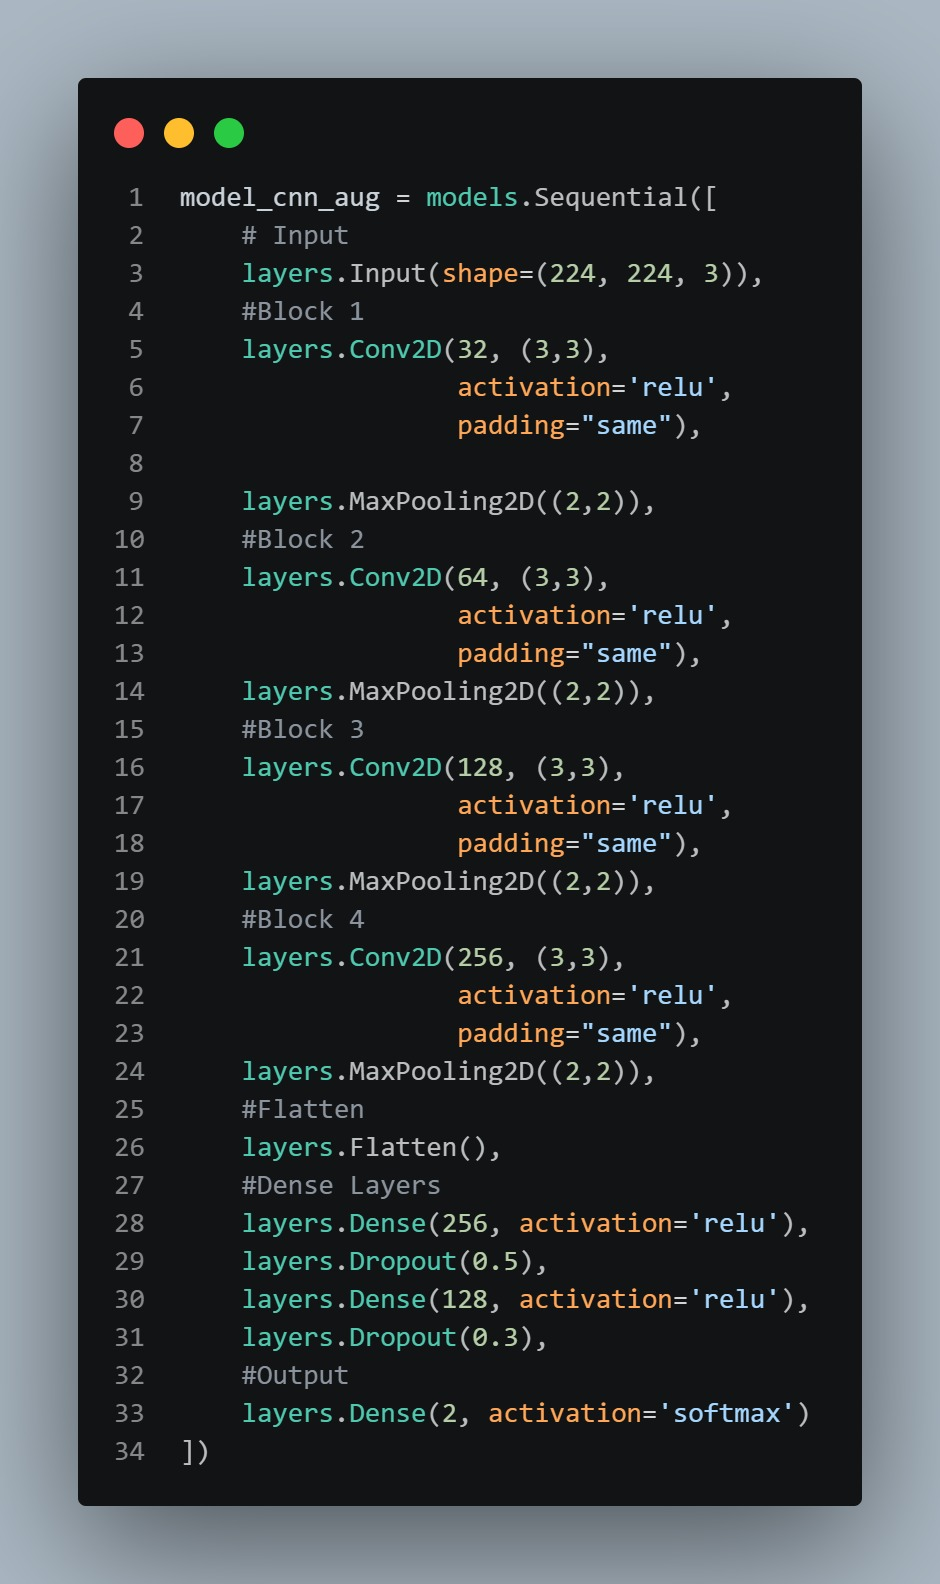
\includegraphics[width=0.8\linewidth]{code5.jpeg}
    \caption{Matrice de confusion}
\end{figure}


\begin{table}[H]
\centering
\caption{Comparaison des architectures CNN\_REG vs CNN\_AUG}
\label{tab:arch_comparison}
\renewcommand{\arraystretch}{1.3}
\begin{tabular}{|l|c|c|}
\hline
\textbf{Composant} & \textbf{CNN\_REG} & \textbf{CNN\_AUG} \\
\hline
Blocs Conv (×4)          & Conv + BN + ReLU + MaxPool & Conv + ReLU + MaxPool \\
\hline
Couches denses           & Dense + BN + ReLU          & Dense + ReLU          \\
\hline
Dropout                  & $0{,}5$ et $0{,}3$         & $0{,}5$ et $0{,}3$    \\
\hline
Batch Normalization      & oui                     & non                \\
\hline
Augmentation de données  & non                     & oui (12 transformations) \\
\hline
Early stopping patience  & 3                          & 5                     \\
\hline
\end{tabular}
\end{table}


\subsection{Courbes d'apprentissage}

\begin{figure}[H]
\centering
    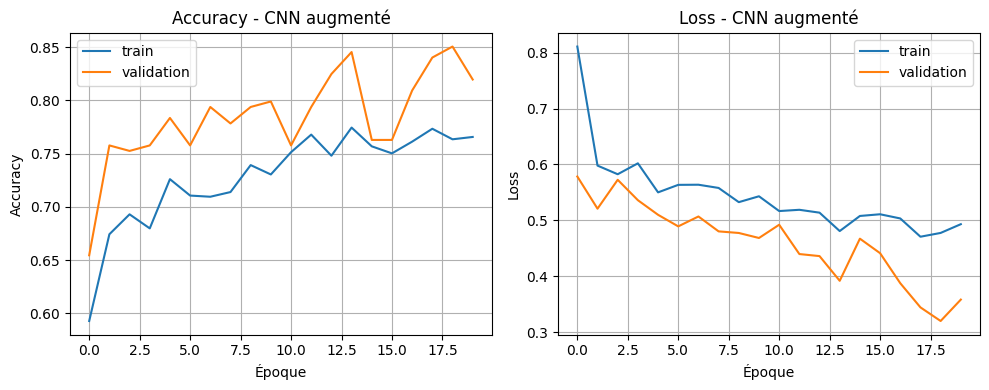
\includegraphics[width=0.8\linewidth]{code6.png}
    \caption{Courbes d'apprentissage}
\end{figure}

\subsubsection{Lecture des courbes}
- La courbe train (bleue) démarre à ~0,60 à l'époque 0, progresse lentement et de manière irrégulière, pour atteindre ~0,77 à l'époque 19.

- La courbe validation (orange) démarre plus haut à ~0,65, oscille entre 0,75 et 0,85 tout au long de l'entraînement, avec un pic maximal de ~0,85 vers l'époque 13–14, avant de légèrement redescendre à ~0,82 en fin d'entraînement.

- La loss d'entraînement (bleue) démarre à ~0,80, décroît progressivement avec des oscillations, pour se stabiliser autour de ~0,49 à l'époque 19.

- La loss de validation (orange) démarre à ~0,58, décroît de manière plus régulière et plus rapide que la loss d'entraînement, atteignant un minimum de ~0,32 vers l'époque 18–19.

\subsubsection{Interprétation :}

- Le phénomène le plus remarquable est que la courbe de validation est systématiquement supérieure à la courbe d'entraînement sur la quasi-totalité des époques. Ceci est un comportement inverse du sur-apprentissage classique, directement causé par l'augmentation de données : les images d'entraînement sont présentées sous des formes aléatoirement transformées (flips, rotations, jitter colorimétrique, etc.), rendant la tâche d'entraînement artificiellement plus difficile que l'évaluation sur des images non augmentées.

- La progression lente et irrégulière de la courbe train (oscillations) est également caractéristique de l'augmentation stochastique : chaque époque présente des exemples différents, introduisant de la variance dans le gradient.

- L'absence de divergence entre les deux courbes confirme que le sur-apprentissage est bien contrôlé grâce à l'augmentation.

- Comme pour l'accuracy, la loss de validation est inférieure à la loss d'entraînement sur toute la durée, confirmant l'effet de l'augmentation qui rend l'entraînement plus difficile que l'évaluation.

- La décroissance continue et régulière de la loss de validation, sans divergence ni remontée brutale (contrairement au modèle sans augmentation), est le signe d'une généralisation saine et stable.

- L'écart croissant entre les deux courbes de loss en fin d'entraînement indique que le modèle continue d'apprendre et de progresser sans saturer, suggérant qu'un entraînement plus long (au-delà de 20 époques) pourrait encore améliorer les performances.

\subsubsection{ Conclusion générale :}

Les courbes d'apprentissage du CNN augmenté présentent un profil radicalement différent du modèle sans augmentation. L'augmentation de données remplit parfaitement son rôle de régularisateur fonctionnel : elle élimine le sur-apprentissage, stabilise la validation sur 20 époques et permet d'atteindre une accuracy de 84,26\% contre 80,20\% pour le modèle précédent. En contrepartie, la convergence est plus lente et nécessite davantage d'époques, justifiant la patience d'Early Stopping portée à 5 pour ce modèle.


\subsection{Résultats sur l'ensemble de test}

\begin{table}[H]
\centering
\caption{Résultats d'évaluation du modèle CNN avec augmentation sur l'ensemble de test}
\label{tab:test_results_aug}
\begin{tabular}{|l|c|}
\hline
\textbf{Métrique} & \textbf{Valeur} \\
\hline
Test Loss     & $31{,}68\%$ \\
\hline
Test Accuracy & $84{,}26\%$ \\
\hline
\end{tabular}
\end{table}

\subsection{Matrice de confusion}
\begin{figure}[H]
\centering
    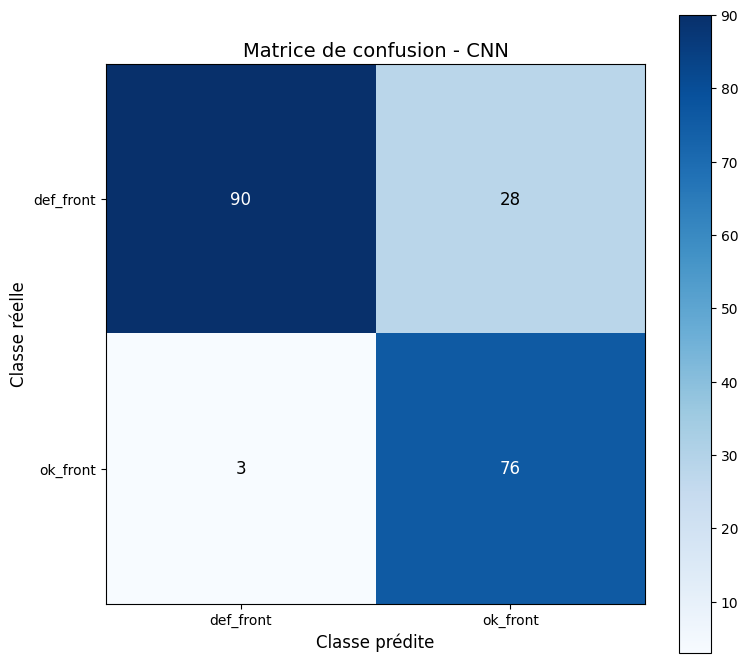
\includegraphics[width=0.8\linewidth]{code7.png}
    \caption{Matrice de confusion du modèle CNN avec augmentation des données}
\end{figure}

\subsection{Rapport de classification}

\begin{table}[H]
\centering
\caption{Rapport de classification — CNN avec augmentation de données}
\label{tab:report_aug}
\renewcommand{\arraystretch}{1.3}
\begin{tabular}{|l|c|c|c|c|}
\hline
\textbf{Classe} & \textbf{Précision} & \textbf{Rappel} & \textbf{F1-Score} & \textbf{Support} \\
\hline
\texttt{def\_front}      & $0{,}97$ & $0{,}76$ & $0{,}85$ & 118 \\
\hline
\texttt{ok\_front}       & $0{,}73$ & $0{,}96$ & $0{,}83$ & 79  \\
\hline\hline
\textbf{Accuracy}        & \multicolumn{3}{c|}{$0{,}84$} & 197 \\
\hline
\textbf{Macro avg}       & $0{,}85$ & $0{,}86$ & $0{,}84$ & 197 \\
\hline
\textbf{Weighted avg}    & $0{,}87$ & $0{,}84$ & $0{,}84$ & 197 \\
\hline
\end{tabular}
\end{table}

% =============================================================
\section{Comparaison des Deux Modèles}
% =============================================================

\begin{table}[H]
\centering
\caption{Comparaison des performances finales sur l'ensemble de test}
\label{tab:comparison}
\renewcommand{\arraystretch}{1.4}
\begin{tabular}{|l|c|c|}
\hline
\textbf{Critère} & \textbf{CNN régularisé} & \textbf{CNN + Augmentation} \\
\hline
Accuracy test               & $80{,}20\%$         & $84{,}26\%$ \\
\hline
Amélioration absolue        & ---                 & $+4{,}06$ pp \\
\hline
Amélioration relative       & ---                 & $+5{,}06\%$ \\
\hline
Régularisation structurelle & BN + Dropout        & Dropout seulement \\
\hline
Augmentation de données     & Non                 & Oui (12 transformations) \\
\hline
Early stopping patience     & 3                   & 5 \\
\hline
\end{tabular}
\end{table}


\subsection{Visualisation comparative}


\begin{figure}[H]
\centering
    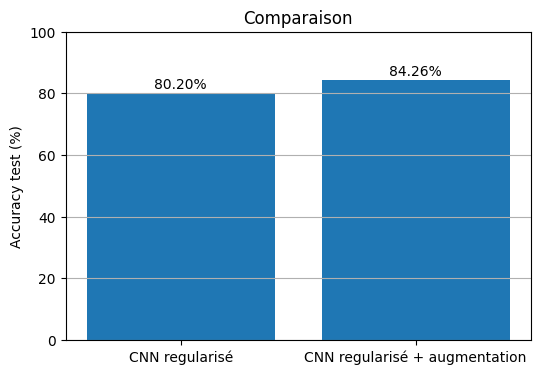
\includegraphics[width=0.8\linewidth]{code8.png}
    \caption{Comparaison des deux modèles}
\end{figure}

Le diagramme en barres  illustre clairement
l'apport de l'augmentation de données : une amélioration de
\textbf{4{,}06 pourcentage} en l'accuracy sur l'ensemble de test.


\subsection{Analyse qualitative}

\begin{table}[H]
\centering
\caption{Analyse qualitative comparative des deux approches}
\label{tab:qualitative}
\renewcommand{\arraystretch}{1.3}
\begin{tabular}{|p{5cm}|p{4.5cm}|p{4.5cm}|}
\hline
\textbf{Aspect} & \textbf{CNN régularisé} & \textbf{CNN + Augmentation} \\
\hline
Régularisation & BN comme régularisateur implicite fort & Augmentation comme régularisateur externe \\
\hline
Vitesse de convergence & Rapide (BN) & Plus lente (variabilité aug.) \\
\hline
Stabilité validation & Bonne & Très bonne \\
\hline
Robustesse aux perturbations & Modérée & Haute \\
\hline
Coût computationnel & Modéré & Plus élevé (aug. en ligne) \\
\hline
Performance finale & $80{,}20\%$ & $84{,}26\%$ \\
\hline
\end{tabular}
\end{table}
\section{Discussion}

L'amélioration de \textbf{+4{,}06\%} apportée par l'augmentation de données
peut s'expliquer par plusieurs mécanismes :

\begin{enumerate}
  \item \textbf{Augmentation artificielle de la diversité} : chaque image est
        présentée sous des centaines de variantes au fil des époques, forçant
        le réseau à apprendre des caractéristiques invariantes à l'orientation,
        l'éclairage et la couleur ;

  \item \textbf{Spécificité industrielle des transformations} : les transformations
        comme l'AWB, l'égalisation d'histogramme et le channel shuffle ont été
        conçues pour refléter les conditions réelles d'acquisition d'images en
        usine (variabilité de l'éclairage, caméras différentes) ;

  \item \textbf{Réduction du sur-apprentissage} : l'augmentation agit comme un
        régularisateur fonctionnel qui complète le Dropout, rendant le modèle
        moins sensible aux artefacts spécifiques du jeu d'entraînement.
\end{enumerate}